% !TEX TS-program = XeLaTeX
% use the following command:
% all document files must be coded in UTF-8
\documentclass[english]{textolivre}
% build HTML with: make4ht -e build.lua -c textolivre.cfg -x -u article "fn-in,svg,pic-align"

\journalname{Texto Livre}
\thevolume{15}
%\thenumber{1} % old template
\theyear{2022}
\receiveddate{\DTMdisplaydate{2022}{7}{17}{-1}} % YYYY MM DD
\accepteddate{\DTMdisplaydate{2022}{8}{23}{-1}}
\publisheddate{\today}
\corrauthor{Adriana E. Mónico Bordino}
\articledoi{10.35699/1983-3652.2022.40501}
%\articleid{NNNN} % if the article ID is not the last 5 numbers of its DOI, provide it using \articleid{} commmand 
% list of available sesscions in the journal: articles, dossier, reports, essays, reviews, interviews, editorial
\articlesessionname{dossier}
\runningauthor{Mónico Bordino} 
%\editorname{Leonardo Araújo} % old template
\sectioneditorname{Daniervelin Pereira}
\layouteditorname{Carolina Garcia}

\title{SEM model in neuromarketing as a planning tool in higher education}
\othertitle{Modelo SEM em \textit{neuromarketing} como uma ferramenta de planejamento no ensino superior}
% if there is a third language title, add here:
%\othertitle{Artikelvorlage zur Einreichung beim Texto Livre Journal}

\author[1]{Adriana Estefania Mónico Bordino \orcid{0000-0003-2287-3833} \thanks{Email: \href{mailto:monico.adriana@gmail.com}{monico.adriana@gmail.com}}}
\affil[1]{Universidad Americana, Escuela de Posgrado, Asunción, Paraguay.}

\addbibresource{article.bib}
% use biber instead of bibtex
% $ biber article

% used to create dummy text for the template file
\definecolor{dark-gray}{gray}{0.35} % color used to display dummy texts
\usepackage{lipsum}
\SetLipsumParListSurrounders{\colorlet{oldcolor}{.}\color{dark-gray}}{\color{oldcolor}}

% used here only to provide the XeLaTeX and BibTeX logos
\usepackage{hologo}

% if you use multirows in a table, include the multirow package
\usepackage{multirow}

% provides sidewaysfigure environment
\usepackage{rotating}

% CUSTOM EPIGRAPH - BEGIN 
%%% https://tex.stackexchange.com/questions/193178/specific-epigraph-style
\usepackage{epigraph}
\renewcommand\textflush{flushright}
\makeatletter
\newlength\epitextskip
\pretocmd{\@epitext}{\em}{}{}
\apptocmd{\@epitext}{\em}{}{}
\patchcmd{\epigraph}{\@epitext{#1}\\}{\@epitext{#1}\\[\epitextskip]}{}{}
\makeatother
\setlength\epigraphrule{0pt}
\setlength\epitextskip{0.5ex}
\setlength\epigraphwidth{.7\textwidth}
% CUSTOM EPIGRAPH - END

% LANGUAGE - BEGIN
% ARABIC
% for languages that use special fonts, you must provide the typeface that will be used
% \setotherlanguage{arabic}
% \newfontfamily\arabicfont[Script=Arabic]{Amiri}
% \newfontfamily\arabicfontsf[Script=Arabic]{Amiri}
% \newfontfamily\arabicfonttt[Script=Arabic]{Amiri}
%
% in the article, to add arabic text use: \textlang{arabic}{ ... }
%
% RUSSIAN
% for russian text we also need to define fonts with support for Cyrillic script
% \usepackage{fontspec}
% \setotherlanguage{russian}
% \newfontfamily\cyrillicfont{Times New Roman}
% \newfontfamily\cyrillicfontsf{Times New Roman}[Script=Cyrillic]
% \newfontfamily\cyrillicfonttt{Times New Roman}[Script=Cyrillic]
%
% in the text use \begin{russian} ... \end{russian}
% LANGUAGE - END

% EMOJIS - BEGIN
% to use emoticons in your manuscript
% https://stackoverflow.com/questions/190145/how-to-insert-emoticons-in-latex/57076064
% using font Symbola, which has full support
% the font may be downloaded at:
% https://dn-works.com/ufas/
% add to preamble:
% \newfontfamily\Symbola{Symbola}
% in the text use:
% {\Symbola }
% EMOJIS - END

% LABEL REFERENCE TO DESCRIPTIVE LIST - BEGIN
% reference itens in a descriptive list using their labels instead of numbers
% insert the code below in the preambule:
%\makeatletter
%\let\orgdescriptionlabel\descriptionlabel
%\renewcommand*{\descriptionlabel}[1]{%
%  \let\orglabel\label
%  \let\label\@gobble
%  \phantomsection
%  \edef\@currentlabel{#1\unskip}%
%  \let\label\orglabel
%  \orgdescriptionlabel{#1}%
%}
%\makeatother
%
% in your document, use as illustraded here:
%\begin{description}
%  \item[first\label{itm1}] this is only an example;
%  % ...  add more items
%\end{description}
% LABEL REFERENCE TO DESCRIPTIVE LIST - END


% add line numbers for submission
%\usepackage{lineno}
%\linenumbers

\begin{document}
\maketitle

\begin{polyabstract}
\begin{abstract}
The purpose of this research is to analyze the relationship between marketing, neuromarketing and strategic planning at the university level. This study is based on a quantitative methodology with an interpretative paradigm, through a non-experimental, transectional, explanatory, descriptive and correlational research design.  For this purpose, a Likert scale was elaborated for 616 students and graduates of the careers offered at the 25 de Mayo Campus of the Universidad Columbia del Paraguay. The analysis was carried out through a Pearson's r correlation, a descriptive analysis and an exploratory factor analysis (SEM), concluding that it is necessary to develop educational marketing actions with different approaches to the current ones. If the educational institution wants to be competitive, it has to strengthen actions to attract potential students through techniques that are competitive in today's society, and that is where neuromarketing comes in. The SEM model allows us to conclude that there is a relationship between university, educational marketing, neuromarketing, quality higher education and strategic planning, highlighting that strategic planning is the key to quality higher education, and that in the educational field marketing should be based on neuromarketing, although it is not yet an indicator of quality higher education.

\keywords{Neuromarketing \sep Educational marketing \sep Strategic planning \sep SEM}
\end{abstract}

\begin{portuguese}
\begin{abstract}
O objetivo desta pesquisa é analisar a relação entre \textit{marketing}, \textit{neuromarketing} e planejamento estratégico a nível universitário. Este estudo é baseado em uma metodologia quantitativa com um paradigma interpretativo, através de um projeto de pesquisa não-experimental, transeccional, explicativo, descritivo e correlacional. Para esse fim, foi elaborada uma escala Likert para 616 estudantes e graduados das carreiras oferecidas no Campus 25 de Mayo da Universidad Columbia del Paraguay. A análise foi realizada através de uma correlação r Pearson, uma análise descritiva e uma análise exploratória de fatores (SEM), concluindo que é necessário desenvolver ações de \textit{marketing} educacional com abordagens diferentes das atuais. Se a instituição educacional quer ser competitiva, tem que fortalecer ações para atrair estudantes potenciais através de técnicas que sejam competitivas na sociedade atual, e é aí que entra o \textit{neuromarketing}. O modelo SEM nos permite concluir que existe uma relação entre universidade, \textit{marketing} educacional, \textit{neuromarketing}, educação superior de qualidade e planejamento estratégico, destacando que o planejamento estratégico é a chave para uma educação superior de qualidade, e que no campo educacional o \textit{marketing} deve ser baseado no \textit{neuromarketing}, embora ainda não seja um indicador de educação superior de qualidade.

\keywords{\textit{Neuromarketing} \sep \textit{Marketing} educacional \sep Planejamento estratégico \sep SEM}
\end{abstract}
\end{portuguese}
% if there is another abstract, insert it here using the same scheme
\end{polyabstract}

\section{Introduction}

The purpose of this research is to analyze the relationship between marketing, neuromarketing and strategic planning in the university environment. The Columbia University of Paraguay -Sede 25 de Mayo - has been used for data collection. From this data, we tried to identify the advertising indicators, with the purpose of determining the stimuli and incentives that induce a certain reaction of the student (potential client) before a purchase decision, (in this case the selection of a private university), in order to extract new conclusions of practical application in the elaboration and design of advertising messages that favor the selection of the university during the decision making process. Thus, marketing, neuromarketing and strategic planning are the topics of this research.

This research proposal arises from two complementary ideas that are, on the one hand, the result of a constant concern to seek a convergence between the normative content (theory) and the practice in educational marketing, which facilitates the construction of a set connected between the two in order to improve the way in which the academic offer is carried out at private universities in the Republic of Paraguay. The first idea states that marketing should be conceived as a philosophy of the organization's activity, whatever its field, and this philosophy is intended to guide managers and thus understand it as a set of techniques that are applied to increase sales or, in the case of this research, student enrollment and retention. The second is based on the company's effective understanding of how consumers respond to the different characteristics of the service offered not only to pricing strategies, but also to advertisements and the media used, as well as the factors that most influence the selection of one offer or -another- in this case, the selection of a private university for an undergraduate degree. This management involves satisfying customer desires as the best means of achieving growth and profitability objectives \cite{lambin_strategic_1992}. Researchers have invested heavily in understanding the relationships between marketing stimuli and consumer responses \cite{kotler_marketing_2009}.

On the other hand, marketing operations are the last disciplines of organizational management that have been the subject of scientific research. The variables used in marketing processes do not have clear quantitative properties that can be recognized in production and financial processes. A mathematician defines marketing complexity as causing nonlinear, delayed, interactive, stochastic relationships \cite{kotler_marketing_2009}. Given the various complexities associated with marketing activity, the next question are how to make good decisions, and how to estimate what the response to them will be, knowing that the marketing effort acts through a network of highly unpredictable behavioral relationships. It should be added that the market's response to this effort is also subject to the events of general economic movements and the incursions of the competition.

\textcite{drucker_practice_1954} states that marketing is not a department; it is the company as a whole seen from the customer's point of view. With this definition it can be considered that the creation of value for the customer should be the competence of all the people working within the organization and not exclusively of the marketing staff. In educational marketing, it does not only pursue the increase of turnover or visibility; it has a much deeper purpose, which is the continuous improvement of the product offered, obtaining a strategic vision and aiming at differentiation from the competition. Another important objective is to build loyalty and generate a sense of belonging, creating experiences and moments that are unforgettable for our consumers. If the university is able to generate this feeling, students and graduates will be the best marketing element the institution can count on. Another very important element is visibility, creating notoriety outside the academic institution, which is why we must take into account the creation of communication campaigns with impact, to preserve the image that the educational institution wishes to transmit.

The concept of \textit{customer experience} has been gaining strength in recent years, taking into account that the marketing strategy has migrated from the company to the people, focusing on customer experience processes. In the educational field, the student or customer bases his experience on the learning process that he/she lives throughout the university career or professional training. Thus, it is important to be able to take information from the environment, in order to generate a product that can meet the needs of users. There are three levels from which information can be obtained for the definition of the product: society, educational sector and customers \cite{llorente_alonso_marketing_2017}.

\textcite{llorente_alonso_marketing_2017} mentions that society will offer a vision of the world in which it currently belongs. Here it will be possible to observe trends, social movements, technological advances, the new supply of products and services, as well as the economic cycles of the groups targeted by the educational institution. On the other hand, the educational sector will offer information on what is happening in other educational institutions, not only locally, but globally. It should not be forgotten that nowadays there is global competition for access to information and the internationalization of education. From this sector, it is possible to obtain information on trends, innovation in the teaching-learning process, new tools that facilitate the different processes of the educational institution, as well as the recruitment of new teachers who can teach in the institution. The third level is the clients, i.e., the students. Surveys, \textit{focus groups} and internal market studies are very important for the educational institution to know its strengths, work on its weaknesses and adapt to the needs or demands of its customers, which will not be very different from the needs of potential customers, i.e., those potential future students it wishes to attract.

The neurosciences were incorporated as a tool in the area of knowledge within psychology and economics. The main reason for this incorporation is to understand the relationship that may exist between the mind and the body of the human being; to analyze the cells that are connected, forming systems that in turn generate the sensory perceptions of the human being in their daily activities, thus providing an answer for marketing actions that seek to understand consumer behavior and the factors that affect their purchase \cite{malfitano_neuromarketing._2016}.  In recent years has emerged in all countries the term of neuroeducation, within the most recent teaching methods currently appear immersed in this new science, which is understood as a new line of thought and action whose primary objective is to bring educators closer to knowledge related to the brain and learning \cite{hernandez_relation_2020} The study of consumer behavior from neuroscience is also called consumer neuroscience. Neurosciences have contributed to the study of consumer behavior, contributing to the knowledge of standards in emotions, taking advantage of user information to generate customer loyalty and rewards processes and thus also capturing potential customers (people who have not yet purchased or consumed the good or service offered). This fusion of neurosciences and business sciences has allowed companies or institutions to know their customers, their emotions, what they feel, what they want and, above all, what they think, in order to generate a process of loyalty and preference. Consumer behavior in neuroscience is mainly classified into four types: decision making, reward, memory and generation of emotions \cite{solnais_contribution_2013} characterized as the main driver of its neurotransmitters, such as serotonin, dopamine and oxytocin.

Neuromarketing is a discipline that uses techniques based on scientific principles and investigates the way in which people think and make decisions; a process that happens most of the time unconsciously. The beginning of neuromarketing arises from the concern for customer service, quality, loyalty and brand loyalty, which would later be lost with the economic crisis in the 1990s in the United States \cite{jones_historical_1990}. Prior to this concept, marketing based its activities on the four P's or Marketing Mix, Jerome McCarthy's Theory \cite{mccarthy_basic_1964}: Product, Price, Place, Promotion. A year later, the concept of the four C's, a customer-oriented concept, was introduced. \textcite{lauterborn_new_1990}, suggests a consumer-oriented version, in which he integrates mass marketing, focusing it on market niches, taking into account the cost, expectations, communication and convenience of the user or customer. The impulses of neuromarketing came to complement the daily life of the human being, for example, the use of colors or colorimetry to generate different sensations on a product, environment or commercial premises. Other examples could be: background or ambient music, smells, characters or \textit{influencers}, location on the gondola or differentiated space of the product within the store. Although neuromarketing is still considered an experimental science, this science studies the effects that marketing actions, impulses, advertising and other communication actions generate in the human brain; the purpose of this science is to be able to predict consumer behavior. It could be considered a specialized model of market research, which focuses directly on the reactions or feelings generated in the consumer by a marketing or communication action and its influence. Néstor Braidot defines neuromarketing as an advanced discipline that researches and studies the brain processes that explain the behavior and decision-making of people in the fields of action of traditional marketing: market intelligence, product and service design, communications, pricing, branding, positioning, \textit{targeting}, channels and sales \cite{braidot_neuromarketing_2009}. On the other hand, the usefulness of neuromarketing has already been verified, as \textcite{barco_neuromarketing_2021} concluded in their research that there is a moderate and positive relationship between neuromarketing and business for small emerging companies. To sum up, in the words of \textcite{caicedo_bibliometric_2021}, it can be said that neuromarketing is a branch of marketing that is emerging with great force in society, since it is the only branch of knowledge capable of offering objective information about consumers, as it obtains brain data on the unconscious patterns of human beings. Thus, \textcite{lyu_problemas_2021} state that the emergence of neuromarketing has caused some concerns and criticisms in relation to the intrusion of physiological measurement in the study of consumer behavior.  Numerous researchers have highlighted that the use of some of the neuromarketing tools can cause a loss of personal privacy and even lead to discrimination, stigmatization and coercion of specific individuals or groups.

Traditional market research is flawed by a basic neurological factor: what our brains perceive and remember is different from what the person says he or she perceived and remembered. The reason this happens is because during the time in which the information is processed to translate it into a spoken response, the brain alters the primary response.  This is where the technological tools of neuromarketing make a difference by assessing beyond an elaborated response to a stimulus, since the time of the exact and primary reaction is assessed, before the alteration of the response to the stimulus interferes. 

On the other hand, the development of a strategic plan and an operational plan produces benefits such as the development of an efficient task, optimizing the use of material resources and human resources, which leads the organization to an effective optimization of time and resources, achieving productive efficiency. The marketing plan is an important part of any business plan. This section describes in detail the product or intangible asset, its price and pricing, its distribution, but above all, it describes how the product offered by the organization will be promoted. Ricardo Hoyos mentions that the marketing plan is the document that relates the objectives of an organization with the commercial area, with its resources, that is, it is the logbook through which the company establishes which objectives it wants to achieve \cite{hoyos_ballesteros_marketing_2013}. Therefore, the marketing plan can be thought of as the roadmap, the path to be followed, with actions to be implemented, in order to achieve the objectives proposed in the strategic plan.

Throughout the above, there are no studies that relate marketing, neuromarketing and strategic planning at the university level as such, and that explains the need to seek this interrelationship and see what conclusions it brings.

\section{Method}

The general objective of this research is to analyze the relationship between marketing, neuromarketing and strategic planning at the university level. It is based on a non-experimental, descriptive, explanatory and correlational design, quantitative methodology and an interpretative paradigm. In order to carry out the research, a Likert scale was chosen as the research instrument.

For the data collection survey among students, a probabilistic sample was taken, with stratified sampling, since a representative number of students per degree program has taken, performing a proportional allocation, where the number of students is distributed proportionally, according to the population of each stratum or, in this case, of each degree program. In the case of data collection with graduates of the different degree programs offered by the 25 de Mayo Campus, a non-probabilistic snowball sampling was chosen. In this case, some graduates were located, with other graduates until a sufficient sample is obtained. The calculation of the sample of non-graduated students is determined as follows: the population involves students from the 25 de Mayo Campus of the Universidad Columbia del Paraguay in the year 2020. Margin: 5\%. Confidence level: 95\%. Population: 2958. Sample size: 341 participants. The calculation of the graduated students sample is determined as follows: considering the last 5 years 2015-2020. Margin: 5\%. Confidence level: 95\%. Population: 961. Sample size: 275 participants. The total sample is 616 participants (341 students and 275 graduates).

The dimensions we considered in this study, extracted from the theoretical framework and the construction of the Likert scale are A.-University; B.-Marketing and education; C.-Neuromarketing; D.-Higher education and quality; and finally, E.-Strategic planning. The dependent variable is neuromarketing, and the independent variables: higher education, quality and strategic planning. The hypotheses established are H$_0$: There is no relationship between marketing, neuromarketing and strategic planning at university level H$_1$: There is a relationship between marketing, neuromarketing and strategic planning at university level.

The design of the Likert scale was carried out with an operationalization table and the validation was carried out, first of all, with an expert judgment and pilot test, and secondly, a factor analysis was performed to validate the scale in its construct using SPSS v25 software. The reliability analysis was calculated with Cronbach's alpha, giving a score of .905 for the 38 items that make up the scale, which is considered excellent \cite{george_spss_2003}.

\section{Results}

Regarding validity, firstly, content validity was carried out by specialists authorized to perform this evaluation table. The validation belonging to different universities. For the specialists the Knowledge or Information Coefficient (Kc) and the Argumentation Coefficient (Ka) were calculated, and then the value of the Competence Coefficient (K) was calculated to determine which experts are taken into consideration to work in this research, were obtained fifteen specialists with an average K of .9, which shows a high level of competence \cite{mengual_importance_2011}. After analyzing the validation questionnaires, some questions were readjusted, without affecting the substance of the question. Also, a pilot test was carried out on a subgroup of the sample research. We obtained a review comprehension difficulty, identify questions that generated doubt, etc., and the corresponding checklist was used. The results of the pilot test were satisfactory, and the instrument was validated in its content.


\subsection{Construct validity (Exploratory Factor Analysis)}

The factor analysis technique applied in the research is exploratory in nature:

1. Study of the correlation matrix: it is necessary to study the correlation matrix to check if our data are adequate to perform a factor analysis. To do this, the correlation matrix must have a certain structure. In order to check this structure, the Kaiser-Meyer-Olkin measure of sampling adequacy (KMO coefficient) has been used in order to check such structure, in this case the value is .800, following \textcite{kaiser_index_1974}, the value is acceptable, Bartlett's test of sphericity has a significance of .000, and the value of the determinant is $\text{8.563E}^{\text{-9}}$, so we continue with the analysis.

2. Factor extraction: once it has been decided that factor analysis can continued good results, we provide to the extraction of the factors. In a good extraction, these values should be high (the closer to one the better) in all variables. The resulting table of communalities shows that the factors have a value greater than .372, so it is not necessary to eliminate any item from the factor analysis (\Cref{Table01}).

The best represented items are: E32 (.770)-I remember the advertisements that appear in my social networks. D31. (.769)-I remember promotions carried out by private universities. D20. (.764)-The marketing campaigns of Columbia University of Paraguay are efficient. C11. (.729)- The social environment influences the consumer. B7. (.724)-The years of experience of the private university are very important when deciding.

The worst represented item is: A5. (.372)-I chose the university because of its fees.

\begin{table}[h!]
\small
\centering
\caption{\textit{Communities}}
\begin{tabular}{p{0.8\textwidth}ll}
\toprule
A.1. I chose the university because of its location. & 1,000 & ,611 \\
A.2. I chose the University on the recommendation of friends or relatives. & 1,000 & ,678 \\
A.3. Marketing actions are the decisive factor in consumer decision making. & 1,000 & ,605 \\
A.4. I chose the University because of the careers it offers. & 1,000 & ,546 \\
A.5. I chose the University because of its fees. & 1,000 & ,372 \\
B.6. The education and culture of young people influence the way in which the communication campaigns of the different private universities are understood. & 1,000 & ,665 \\
B.7. The years of track record of the private university are very important when deciding. & 1,000 & ,724 \\
B.8. Institutional image influences university selection, whether private or public. & 1,000 & ,637 \\
B.9. A good educator is a good marketing professional. & 1,000 &	,669 \\
B.10. A marketing professional is an education professional. &	1,000 & ,717 \\
C.11. The social environment influences the consumer & 1,000 & ,729 \\
C.12. Cultural environment influences the consumer & 1,000 & ,678 \\
C.13. Sensory and perceptual factors are decisive in decision making. & 1,000 & ,520 \\
C.14. The effects of purchase or use experiences are decisive in decision making. & 1,000 & ,636 \\
C.15. Emotional intelligence influences the acceptance and purchase decision of a product. & 1,000 & ,550 \\
C.16. Neural networks generated with previous usage or purchase experiences affect the purchase decision. & 1,000 & ,613 \\
C.17. Neuromarketing actions focused on the brain system of consumers manage to affect their decision-making power.& 1,000 & ,608 \\
D.18. Institutional image influences the decision to enroll in a university. & 1,000 & ,670 \\
D.19. The institutional image reflects quality in the provision of services. & 1,000 & ,711 \\
D.20. The marketing campaigns of Columbia University of Paraguay are efficient. & 1,000 & ,764 \\
D.21. Marketing communications made to student candidates by Universidad Columbia del Paraguay Sede 25 de Mayo are adequate. &	1,000 & ,738\\
D.22. The communications made by Columbia University of Paraguay transmit quality in the education they offer. & 1,000 & ,688 \\
D.23. Years of tenure are synonymous with quality in education. & 1,000 & ,691 \\
D.24. The teaching component of Columbia University is synonymous with quality. & 1,000 & ,649 \\
D.25. Columbia University's infrastructure is synonymous with quality. & 1,000 & ,625 \\
D.26. Student exchange activities, research, participation in outreach activities are synonymous with quality. & 1,000 & ,576 \\
D.27. The 25 de Mayo Campus of Columbia University builds student loyalty. & 1,000 &	,670 \\
D.28. Control and monitoring tools are useful in strategic marketing plans. & 1,000 & ,660 \\
D.29. Private universities need to carry out marketing actions. & 1,000 & ,530 \\
D.30. I find out if the career I am pursuing or wish to study is accredited at the university I am interested in. & 1,000 & ,546 \\
D.31. I recall the promotions carried out by private universities. & 1,000 & ,769 \\
E.32. I remember the advertisements that appear in my social networks. & 1,000 & ,770 \\
E.33. I remember the advertisements that appear in traditional media such as TV, radios, magazines or newspapers. & 1,000 & ,664 \\
E.34. Before advertising, I consider the advice of people I know to be more important when it comes to making decisions. & 1,000 & ,619 \\
E.35. I consider it important for the University to build student loyalty. & 1,000 &	,702 \\
E.36. It is important that the University performs an efficient accompaniment to its students. & 1,000 & ,716 \\
E.37. Seeing and hearing the testimonials of Columbia University students and alumni will give me peace of mind when I decide to enroll in Columbia University. & 1,000 & ,709 \\
E.38. I feel that at Columbia University I will find good classmates and caring and strong professors to help me develop professionally. &	1,000 & ,596 \\
\textit{Extraction method: principal component analysis.}\\
\bottomrule
\end{tabular}
\label{Table01}
\source{Own elaboration.}
\end{table}

\Cref{Table01} shows the values adopted for the different items, with the highest and lowest scores.

3. Factor rotation: there are several methods to perform the rotations according to the optimality criterion. One of them is the Varimax Rotation, which optimizes the factor loadings so as to obtain the most extreme possible factor loadings (high and low). There are rules for determining the most appropriate number of factors to proceeded, for example, the one known as the \textcite{kaiser_index_1974} criterion, which indicates that the principal components whose eigenvalues are greater than unity should be conserved, although the most commonly used criterion is to observe the percentage of total variance explained by each component or factor, and when this reaches a cumulative percentage considered high, in this case the first 10 factors, which explains 64.798\% of the cumulative variance (\Cref{Table02}).

\begingroup
\setlength\tabcolsep{2pt} % default value: 6pt
\small
\begin{table}[h!]
\centering
\caption{\textit{Total variance explained.}}
\begin{tabular}{*{10}{p{0.09\textwidth}}}
\toprule
&
\multicolumn{3}{p{0.27\textwidth}}{Initial eigenvalues}	& 
\multicolumn{3}{p{0.27\textwidth}}{Sums of loads squared by extraction} & \multicolumn{3}{p{0.27\textwidth}}{Sums of loads squared by rotation} \\
\midrule
Compo\-nent & Total & \% variance & Accumu\-lated & Total & \% variance & Accumu\-lated & Total & \% variance & Accumu\-lated \\
\midrule
1 & 9,090 & 23,921 & 23,921 & 9,090 & 23,921 & 23,921 & 3,951 & 10,397 & 10,397 \\
& 3,073 & 8,086 & 32,007 & 3,073 & 8,086 & 32,007 & 3,435 & 9,039 & 19,435 \\
& 2,246 & 5,911 & 37,918 & 2,246 & 5,911 & 37,918 & 2,729 & 7,181 & 26,617 \\
& 1,880 & 4,948 & 42,866 & 1,880 & 4,948 & 42,866 & 2,434 & 6,405 & 33,022 \\
5 & 1,798 & 4,732 & 47,598 & 1,798 & 4,732 & 47,598 & 2,176 & 5,726 & 38,748 \\
& 1,539 & 4,049 & 51,647 & 1,539 & 4,049 & 51,647 & 2,173 & 5,719 & 44,467 \\
& 1,488 & 3,916 & 55,563 & 1,488 & 3,916 & 55,563 & 2,165 & 5,698 & 50,165 \\
& 1,319 & 3,471 & 59,034 & 1,319 & 3,471 & 59,034 & 1,959 & 5,154 & 55,319 \\
& 1,166 & 3,068 & 62,102 & 1,166 & 3,068 & 62,102 & 1,921 & 5,056 & 60,375 \\
& 1,024 & 2,695 & 64,798 & 1,024 & 2,695 & 64,798 & 1,680 & 4,422 & 64,798 \\
& ,997 & 2,623 & 67,420 \\
\bottomrule
\end{tabular}
\label{Table02}
\source{Own elaboration.}
\end{table}
\endgroup

\Cref{Table02} shows the initial eigenvalues and the sum of squared loadings of the extraction of the different factors.

4. Study of the factor scores: subsequently, the component matrix is calculated, and \Cref{Table03} shows the determination of factors and distribution of items according to the highest level of saturation by factors.


\begingroup
\setlength\tabcolsep{2pt} % default value: 6pt
\begin{table}[h!]
\centering
\caption{\textit{Items integrated in each factor}}
\resizebox{\textwidth}{!}{%
\begin{tabular}{lll}
\toprule
Factor & Designation & Items included in each factor of the questionnaire.\\
\midrule
\multirow{5}{*}{I} & A (University) &  A3,A4,A5 \\
& B (Marketing and education) &  B6,B7,B8,B9  \\
& C (Neuromarketing) &  C13,C14,C15,C16,C17 \\ 
& D (Higher education and quality) & D18,D19,D20,D21,D22,D23,D24,D25,D26,D27,D28,D29, D31 \\ 
& E (Strategic Planning) & E32,E33,E34,E35,E36,E37,E38 \\
II	& C (Neuromarketing) & C11,C12<2 ELEMENTS \\
\bottomrule
\end{tabular}
}
\label{Table03}
\source{Own elaboration.}
\end{table}
\endgroup

Cronbach's alpha was then calculated for both factors: Factor 1: .907 (32 items), rating "excellent". Then, Factor 2, having less than three items, can be eliminated, as well as the rest of the factors. Therefore, Factor 1 it’s taken, which presents a reliability similar to that of the original scale itself (.905) with 38 items, resulting in a final scale of 32 items (\Cref{Table03}).

\subsection{Correlation analysis (Pearson's r)}

To perform the correlation, we subjected the Likert scale to the Mann-Whitney U test for two independent samples, which explains that the data follow a normal distribution, so Pearson's r correlation must be used. Analyzing the research items according to their dimensions, the significant correlation (.05) is established between the following variables: Dimension A (Marketing): A1>B10 (.269), A2>C11 (.370), A3>D20 (.512), A4>A3 (.318), A5>E38 (.339). Dimension B (Marketing and Education) - B6>B7 (.396), B7>B8 (.432), B8>D18 (.484), B9<>B10 (.521). Dimension C (Neuromarketing).-C11<>C12 (.743), C13>C14 (.496), C14>C16 (.559), C15>C17 (.468), C16<>C17 (.576). Dimension D (Higher Education and Quality)-D18<>D19 (.551), D20<>D21 (.571), D22>D21 (.516), D23>D19 (.437), D24>E38 (.460), D25>D27 (.503), D26>D28 (.534), D27>D25 (.503), D28>D26 (.534), D29>E35 (.412), D30>E36 (.218), D31>E32 (.511). Dimension E (Strategic Planning).-E32<>E33 (.688), E34<>E35 (.446), E36<>E37(.562), E38>E37 (.505).

\subsection{Descriptive analysis}

Regarding the descriptive analysis, we will highlight, by dimensions, some of the responses of the research subjects that are relevant to appreciate the ideas of the sample group on the subject under investigation.

In dimension A (University) the participants show their opinion "agree" in a general way in the dimension, with a mean of 3.70. Concretely, the participants show "agree" with A4 (4.30). I chose the university because of the careers it offers. Similarly, they are "indifferent" to A1 (3.30), I chose the university because of its location; A2 (3.82), I chose the university because of recommendations from friends or relatives; A3 (3.44) marketing actions are the decisive factor in consumers showed; and finally, A5 (3.62). I chose the university because of its fees.

Dimension B (Marketing and education) subjects generally "agree" with this dimension, with a mean of 3.94. The participants show "agree" in: B6 (3.97). The education and culture of young people include in the way of understanding the communication campaigns...; B7 (418). The years of trajectory of the private university are very important when deciding; B8 (4.41). Institutional image influences university selection; and B9 (3.73). A good educator is a good marketing professional. They are indifferent on: B10 (3.43). A marketing professional is an education professional.

Dimension C (Neuromarketing), the subjects show "agree" with it, with a mean of 4.05. Participants show "agree" in: C11 (4.09). The social environment influences the consumer; C12 (3.98). The cultural environment influences the consumer; C13 (4.15). Sensory and perceptual factors are decisive in decision-making; C14 (4.14). The effects of purchase or use experiences are decisive in decision making; C15 (4.01). Emotional intelligence influences product acceptance and purchase decision; C16 (4.00). Neural networks generated with previous usage or purchase experiences affect the purchase decision; and C17 (3.96). Neuromarketing actions targeting the brain system of consumers succeed in affecting their decision-making power.

Dimension D (Higher education and quality). Participants show "agree" with a mean of 3.82 with this dimension. Subjects are "indifferent" to: D20 (3.47). Columbia University's marketing campaigns are efficient; D21 (3.43). The marketing communications carried out are adequate; D27 (3.51). The 25 de Mayo Campus of Columbia University builds student loyalty; D31 (3.65). I recall the promotions carried out by private universities. Participants "agree" with: D18 (4.30). Institutional image influences the decision to enroll in the university; D19 (3.91). The institutional image reflects the quality of service delivery; D22 (3.74). The communications made by the university convey quality in the education they offer; D23 (3.91). The years of permanence in the market are synonymous with quality in education; D24 (4.05). The teaching component of Columbia University is synonymous with quality; D25 (3.74). Columbia University's infrastructure is synonymous with quality; D26 (4.03). Student exchange activities, research, participation in outreach activities are synonymous with quality; D28 (4.02). Control and monitoring tools are useful in strategic marketing plans; D29 (4.08). Private universities need to carry out marketing actions; and D30 (4.23). I find out if the career I am pursuing or wish to study is accredited at the university I am interested in.

Finally, dimension E (Strategic planning). Subjects are "indifferent" to: E32 (3.64). I remember the advertisements that appear on my social networks; and E33 (3.69). I remember the advertisements that appear on TV, radio...On the other hand, they "agree" with: E34 (4.16). Before advertising, I consider that the advice of people I know is more important when making decisions; E35 (4.31). I think it is important for the university to build student loyalty; E36 (4.53). It is important that the University provides efficient support to its students; E37 (4.19). Seeing and listening to the testimony of students and alumni of the U.C. will give me peace of mind when deciding to enroll in the same; and E38 (4.03). I feel that at the U.C. I will find good classmates and understanding and strong professors to help me develop professionally.

\subsection{Confirmatory factor analysis (SEM)}

Confirmatory factor analysis represents the measurement model as it is desired to confirm the composition of the underlying dimensions. Path analysis represents a second model, since it is desired to estimate the relationships between variables that are directly observed. Structural Equation Modeling (SEM) provides the most robust technical procedures and criteria for validating measurement models under these two assumptions. The SEM methodology consists of a series of phases according to \textcite{kaplan_structural_2000,kline_principles_2005}, which can be summarized in four.

Phase I.-Specification of the Measurement Model. In this stage the latent traits and the dimensions that represent them as variables of interest of a substantive theory are established. This stage is conceptual in nature and formulates the structure of relationships between the latent variables represented by the dimensions of the instrument and the responses to the items of the context questionnaire. The Conceptual Model of the Likert scale obtained from the exploratory factor analysis is composed of 32 observed variables that are grouped into five dimensions.

Phase II.-Identification. Computational Implementation of the System of Structural Equations. To determine if the model is identified, the degrees of freedom (gl) must be calculated, in this case the value is 374 (greater than zero), so we can say that the model is over-identified.

Phase III.-Parameter estimation. The model estimation phase includes a graphical representation of the theoretical-conceptual structure of the instrument under analysis. This representation is the basis for the formulation of the reproduced matrix that will be compared with the derived matrix. For the Likert scale the graphical representation is shown in \Cref{Figure01}.

\begin{figure}[h!]
\centering
\caption{\textit{Graphic representation of the natural measurement model of the Likert scale}.}
\begin{minipage}{1.0\textwidth}
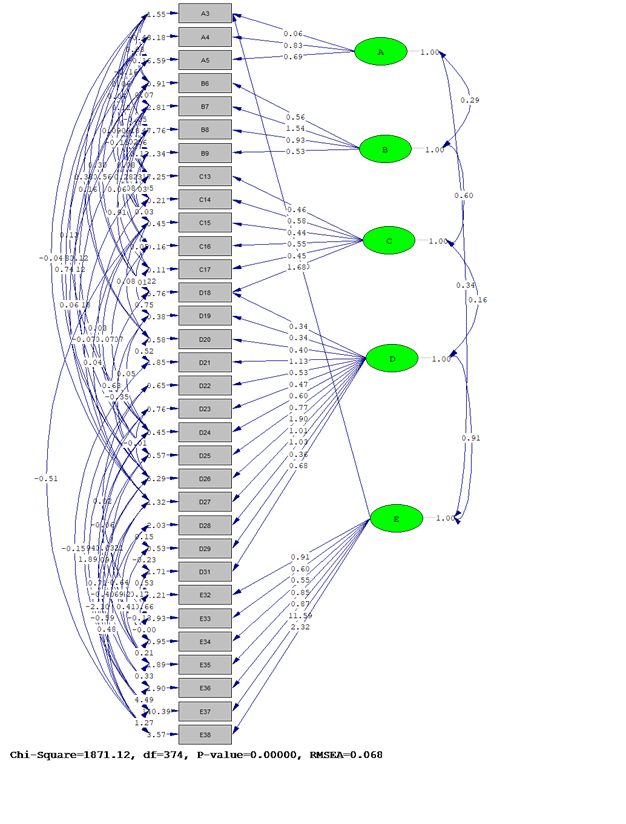
\includegraphics[width=\textwidth]{Figure01.png}
\label{Figure01}
\source{Own elaboration.}
\end{minipage}
\end{figure}

In this phase, the values of the unknown parameters are determined, as well as their respective measurement error. As for the regression coefficients between the latent and observed variables, the interpretation is as follows.

Dimension A (Marketing). Greater influence of the latent variable marketing on A4 (.83).-I chose the university because of the careers it offers. Lower influence of the latent variable on A3 (.06). -. Marketing actions are the decisive factor for consumers' decision making.

Dimension B (Marketing and education). Greater influence of the latent variable on B7 (1.54).-The years of experience of the private university are very important when deciding. Lower influence of the latent variable on B9 (.53). A good educator is a good marketing professional.

Dimension C (Neuromarketing). Greater influence of the latent variable on C14 (.58).-The effects of purchase or use experiences are decisive in decision making. Lower influence of the latent variable on C15 (.44). Emotional intelligence influences the acceptance and purchase decision of a product.

Dimension D (Higher education and quality). Greater influence of the latent variable on D26 (1.90). Student exchange activities, research, participation in extension activities are synonymous with quality. Lower influence of the latent variable Neurodidactics on D18 (.34).-Institutional image influences the decision to enroll in a university. D19 (.34). Institutional image reflects quality in service provision.

Dimension E (Strategic planning). Greater influence of the latent variable on E37 (11.59). Seeing and hearing the testimony of Columbia University students and alumni will give me peace of mind when deciding to enroll in Columbia University. Lower influence of the latent variable Inclusive practices on E34 (.55). Before advertising, I consider the advice of people I know to be more important when making decisions.

The relationship between the latent variables is given by the following values: A (University)-B (Marketing and education) (.29). B (Marketing and education)-C (Neuromarketing) (.60). C (Neuromarketing)-D (Higher Education and Quality) (.16). D (Higher Education and Quality)-E (Strategic Planning) (.91). A (University)-E (Strategic Planning) (.34).

In summary, the strongest relationship between the latent variables is given by: D (Higher education and quality)-E (Strategic planning) (.91) and B (Marketing and education)-C (Neuromarketing) (.60). The lowest relationship is given by: C (Neuromarketing)-D (Higher education and quality) (.16).

Phase IV.-Evaluation of the fit. Application of indices and goodness-of-fit criteria. In this stage we use goodness-of-fit indexes and criteria to relate the validation evidence with the dimensional structure of the instrument being evaluated, (consists of evaluating the goodness-of-fit between the matrix derived from the data and the matrix reproduced by the model: Difference X2/df (1871.12/374), it consist a good indicator if the result ranges between one and three or, more loosely, if the result of the difference is $\leqslant≤5$ \cite{carmines_analyzing_1981,joreskog_general_1970}, the value obtained is 5.00, so the result is good. CFI, compares the improvement in the fit of the model in question with a null model to evaluate the degree of loss of fit when switching from the proposed model to the null model \cite{hu_cutoff_1999}. The value to accept the proposed model, its value should be $\geqslant≥.95.$ To accept the value that results is .96., among the indices based on covariances, the root mean square error of approximation (RMSEA) was chosen. In this case the model would present an acceptable fit if the value was <.07 \cite{steiger_understanding_2007}, the value we calculated in our model is .068 which is acceptable. NNFI reflects the proportion of total information explained by a model; because this index is not standardized, its values can adopt values outside the range 0 and 1. A value of .97 seems to be more reasonable as an indication of good model fit. A value we obtained is .94 \cite[p.~41]{schermelleh_._2003}. As can be seen, the criteria for all goodness-of-fit indices are met, so the model can be considered confirmed.

\section{Discussion and conclusions}

This research was carried out on a population of 616 male and female students and university graduates. The Likert scale was constructed with an operationalization table, and sized, according to the theoretical framework, in five dimensions and 38 items: A.-University; B.-Marketing and education; C.-Neuromarketing: D.-Higher education and quality; and E.-Strategic planning. The objective of this research was to analyze the relationship between marketing, neuromarketing and strategic planning in the university environment. For the validation of the data collection instrument, we resorted to content validation, which was satisfactory, and construct validation, through exploratory factor analysis. The result of this analysis on the one hand confirms our dimensions, and on the other hand reduces the scale to 32 items, obtaining a reliability according to Cronbach's alpha of excellent (. 907), so it is validated in its construct.

The Mann-Whitney U test allows us to determine that the data follow a uniform distribution, and retains the null hypothesis, so we proceed to the correlation analysis with Pearson's P, which allows us to affirm, significantly, that the marketing actions and campaigns of Columbia University are efficient for students' decision making. That a good educator is a good marketing professional who in turn is an education professional. The institutional image influences the decision and selection. That the social and cultural environment influences the consumer. Neuromarketing actions and the neural networks generated influence decision making. Importance of radio, television and newspaper advertising, as well as social networks. It can be observed that marketing actions, the image of the institution, the quality of the faculty and neuromarketing actions with key to the choice of the educational institution. The descriptive analysis shows that the participants, in general terms, "agree" with all the dimensions (although to a greater extent with C (Neuromarketing) and D (Strategic planning), reaffirming the importance of neuromarketing for strategic planning. However, it should be noted that university students and graduates are "indifferent" to the location of the university, the influence of friends or family in the choice, quotas imposed by the university, marketing campaigns and promotions.

The SEM analysis allows us to analyze the data in a deeper way, in relation to marketing, what is most important is the range of careers that the university offers, and what has the least influence are the marketing actions that it can perform. The years of experience of the university is the most influential in relation to marketing and education, and what is least important is whether the professor is a good marketing professional. In relation to neuromarketing, what is most important is the experience acquired and what is least important is the influence of emotional intelligence. Regarding higher education and quality, what is most important are the activities offered by the university, and what is least important is the institutional image. Finally, in relation to strategic planning, what is most important are the testimonies of graduates about their university experience, and what is least important is the advice of people they know. As we can see, the empathy of students with graduates is a neuroscientific factor to be taken into account. Finally, in relation to the established hypotheses, the alternative hypothesis is confirmed as valid, being able to offer that there is a relationship between the investigated elements. In fact, quality higher education has much to do with an optimal strategic planning, marketing in education should be based on neuromarketing, yet understanding that neuromarketing determines quality higher education. In general terms, we confirm the ideas of \textcite{barco_neuromarketing_2021,caicedo_bibliometric_2021} in the sense of the importance of neuromarketing in the choice of institution, just as the motivations of students and graduates in their final choice clarified \cite{lambin_strategic_1992,kotler_marketing_2009,llorente_alonso_marketing_2017}.

Although the research was limited to a case study, it can be the beginning of other broader research that will provide data to government education officials on the particular situation of the context investigated. The research has been carried out, for convenience, with the participation of a sample of students and graduates. In a next research it would be acceptable to carry out this research with students and graduates from other universities, to correlate the data at different levels, as well appropriate the study in education teachers, to appreciate the different perceptions that the different with samples have about neuroeducation.

The research presented analyzed the relationship between marketing, neuromarketing and strategic planning in the university environment, through a sample of 616 students and university graduates from a specific university in Paraguay, Columbia University. A first conclusion that can be drawn is that it is possible to have a scale for obtaining data validated in its construct, which makes it not only valid but also very reliable. From this scale it can also be concluded that the memory of the marketing carried out by the university, as well as the influence of the social environment and the years of trajectory of the institution itself are important, but not decisive in the decision making process, and of course the least important is the price of studying at that institution. Another important conclusion that can be highlighted is that the influence of the institutional image, the power of the communication and mass-media networks, as well as the quality of the institution's teaching staff, must be taken into account when making decisions, and of course, neuromarketing stands out as a key factor in the institution's strategic planning.

However, the most revealing conclusions are provided by the SEM carried out, which confirms the importance of career offerings, years of experience, good teaching professionals, and in relation to neuromarketing, the importance of empathy with graduate students, rather than being carried away by emotions in decision making. It really shows the little importance that the institutional image has for the future student, acquiring greater relevance the offer of activities that the institution can give.

Finally, it can be concluded that there is a relationship between university, educational marketing, neuromarketing, quality higher education and strategic planning, highlighting that strategic planning is the key to quality higher education, and that in the educational field marketing should be based on neuromarketing, although it is not yet an indicator of quality higher education. With all this, it is necessary to develop educational marketing actions with different approaches to the current ones, if the educational institution wants to be competitive, thus having to strengthen actions to attract potential students through techniques that are competitive in today's society, and this is where neuromarketing comes in, always taking into account the recommendations of \textcite{lyu_problemas_2021} on the ethical constraints that it must assume in order not to "manipulate" the brains of future university students.


\printbibliography\label{sec-bib}
% if the text is not in Portuguese, it might be necessary to use the code below instead to print the correct ABNT abbreviations [s.n.], [s.l.]
%\begin{portuguese}
%\printbibliography[title={Bibliography}]
%\end{portuguese}

%full list: conceptualization,datacuration,formalanalysis,funding,investigation,methodology,projadm,resources,software,supervision,validation,visualization,writing,review

\end{document}

